\documentclass[12pt,a4paper]{report}
% Language and font
\usepackage[T1]{fontenc}
\usepackage[utf8]{inputenc}
\usepackage[french, english]{babel}
% Page geometry
\usepackage[a4paper, hmargin=2.5cm, vmargin=2.5cm]{geometry}
% Graphics
\usepackage{graphicx}
% Header/footer control
\usepackage{fancyhdr}
\pagestyle{fancy}
\fancyhf{}
\fancyfoot[R]{\thepage}
\renewcommand{\headrulewidth}{0pt}
% Title formatting (optional)
\usepackage{titlesec}
\titleformat{\chapter}[block]
{\normalfont\Huge\bfseries}
{\chaptertitlename\ \thechapter~:}
{20pt}
{\Huge}
\titlespacing*{\chapter}{0pt}{30pt}{12pt}
\titlespacing*{\section}{0pt}{30pt}{12pt}
% For spacing
\usepackage{setspace}
\singlespacing
\parskip=6pt
% Colors (for logos or text if needed)
\usepackage{xcolor}
% For minipages and alignment
\usepackage{tabularx}
% Hyperlinks (optional)
\usepackage[hidelinks]{hyperref}
\usepackage{caption}
\usepackage{subcaption}
\usepackage{float}

\begin{document}
\begin{center}
\rule{1\linewidth}{1pt}
\end{center}
\begin{center}
\begin{minipage}{.1\textwidth}
\includegraphics[scale=0.2]{./ESI.png}
\end{minipage}%
\hfill
\begin{minipage}{.85\textwidth}
\begin{center}
RÉPUBLIQUE ALGÉRIENNE DÉMOCRATIQUE ET POPULAIRE\
MINISTÈRE DE L'ENSEIGNEMENT SUPÉRIEUR ET DE LA RECHERCHE SCIENTIFIQUE\
ÉCOLE NATIONALE SUPÉRIEURE D'INFORMATIQUE
\end{center}
\end{minipage}%
\end{center}
\begin{center}
\rule{1\linewidth}{1pt}
\end{center}
\vspace*{3cm}
\begin{center}
{\Large \textbf{Rapport de TP - ANAD}}
\vspace*{0.5cm}

{\Large 2\up{ème} Année Cycle Supérieur (2CS)\\
Module : Analyse de Données et Fouilles de Données}
\end{center}
\vspace*{1cm}
\begin{center}
\hrule
\vspace*{0.5cm}
{\Large \textbf{\parbox{0.9\linewidth}{Analyse en Composantes Principales et Analyse des Correspondances Multiples}}}
\vspace*{0.5cm}
\hrule
\end{center}
\vspace*{2cm}
\begin{minipage}[t]{0.45\textwidth}
\centering
\textbf{Réalisé par :}\[0.5cm]
\begin{tabular}{l}
ATTIA Oussama Abderraouf \
SRAICH Imene
\end{tabular}
\end{minipage}%
\hfill
\begin{minipage}[t]{0.45\textwidth}
\centering
\textbf{Encadré par :}\[0.5cm]
BOUDI ABDERRAHMAN
\end{minipage}
\vspace*{2cm}
\begin{center}
Année universitaire : 2025--2026
\end{center}
\thispagestyle{empty}

\newpage

% ============================================================================
% RÉSUMÉ EXÉCUTIF
% ============================================================================
\section*{Résumé Exécutif}

Ce rapport présente une analyse multivariée complète d'une base de données comprenant 533 individus et 11 variables (4 quantitatives et 7 qualitatives). L'étude combine l'Analyse en Composantes Principales (ACP) pour explorer les variables quantitatives et l'Analyse des Correspondances Multiples (ACM) pour analyser les associations entre variables qualitatives. Les résultats mettent en évidence les facteurs déterminants des salaires et les structures d'association entre les caractéristiques socio-professionnelles des individus.

\tableofcontents

\newpage

% ============================================================================
% 1. INTRODUCTION
% ============================================================================
\section{Introduction}

\subsection{Contexte et Objectifs}

L'analyse de données est l'une des disciplines fondamentales de la science des données et de la statistique moderne. Ce travail pratique s'inscrit dans le contexte de la Maîtrise en Informatique à l'École Nationale Supérieure d'Informatique (ESI). L'objectif principal est d'appliquer les méthodes d'analyse multivariée sur une base de données réelle comportant plusieurs variables de natures différentes.

\subsection{Objectifs Spécifiques}

\begin{enumerate}
    \item Charger et explorer une base de données réelle avec variables quantitatives et qualitatives
    \item Appliquer l'Analyse en Composantes Principales (ACP) pour réduire la dimensionnalité
    \item Appliquer l'Analyse des Correspondances Multiples (ACM) pour étudier les associations
    \item Interpreter les résultats et extraire des conclusions pertinentes
    \item Fournir visualisations et résumés statistiques complets
\end{enumerate}

\subsection{Respect des Consignes du TP}

Nous avons respecté l'énoncé du travail pratique en conformité complète :

\begin{itemize}
    \item \textbf{Données} : 533 individus (dépassant le minimum de 200)
    \item \textbf{Variables qualitatives} : 7 variables (dépassant le minimum de 4)
    \item \textbf{Modalités} : Plus de 2 modalités pour 6 variables qualitatives
    \item \textbf{Variables quantitatives} : 4 variables (wage, education, experience, age)
    \item \textbf{Format rapport} : Rapport de 10 pages avec interprétation détaillée des résultats
    \item \textbf{Organisation} : Travail réalisé en binôme (ATTIA OUSSAMA ABADERRAOUF et SRAICH IMENE)
\end{itemize}

% ============================================================================
% 2. DESCRIPTION DE LA BASE DE DONNÉES
% ============================================================================
\section{Description de la Base de Données}

\subsection{Provenance et Caractéristiques Générales}

La base de données analysée contient des informations sur le marché du travail, regroupant des données socio-économiques importantes :

\begin{itemize}
    \item \textbf{533 observations} (individus actifs)
    \item \textbf{11 variables} au total
    \item \textbf{4 variables quantitatives} : wage, education, experience, age
    \item \textbf{7 variables qualitatives} : ethnicity, region, gender, occupation, sector, union, married
    \item \textbf{Qualité} : Base complète, aucune valeur manquante détectée
\end{itemize}

\subsection{Variables Quantitatives}

\begin{table}[H]
\centering
\caption{Variables quantitatives - Caractéristiques}
\begin{tabular}{|l|p{3.5cm}|c|c|c|c|}
\hline
\textbf{Variable} & \textbf{Description} & \textbf{Minimum} & \textbf{Moyenne} & \textbf{Maximum} & \textbf{Écart-type} \\
\hline
wage & Salaire horaire & 3.35\$ & 9.02\$ & 25.20\$ & 5.48 \\
\hline
education & Années d'études & 6 ans & 11.56 ans & 17 ans & 2.54 \\
\hline
experience & Expérience prof. & 0 ans & 17.82 ans & 47 ans & 12.71 \\
\hline
age & Âge & 18 ans & 36.83 ans & 64 ans & 11.41 \\
\hline
\end{tabular}
\end{table}

\subsection{Variables Qualitatives}

\begin{table}[H]
\centering
\caption{Variables qualitatives - Informations}
\begin{tabular}{|l|p{4cm}|p{5cm}|}
\hline
\textbf{Variable} & \textbf{Type} & \textbf{Modalités} \\
\hline
ethnicity & Nominale & Caucasien, Hispanique, Autre (3 modalités) \\
\hline
region & Nominale & Sud, Autre (2 modalités) \\
\hline
gender & Binaire & Masculin, Féminin (2 modalités) \\
\hline
occupation & Nominale & Ouvrier, Manager, Ventes, etc. (3+ modalités) \\
\hline
sector & Nominale & Manufacturier, Construction, Services, etc. (4+ modalités) \\
\hline
union & Binaire & Oui, Non (2 modalités) \\
\hline
married & Binaire & Oui, Non (2 modalités) \\
\hline
\end{tabular}
\end{table}

% ============================================================================
% 3. MÉTHODOLOGIE
% ============================================================================
\section{Méthodologie}

\subsection{Analyse en Composantes Principales (ACP)}

L'ACP est une technique de réduction de dimensionnalité qui transforme un ensemble de variables corrélées en un ensemble de variables non-corrélées appelées composantes principales. Elle maximise la variance conservée avec le nombre minimal de dimensions.

\textbf{Objectifs de l'ACP dans cette étude :}
\begin{enumerate}
    \item Réduire les 4 variables quantitatives à un petit nombre de composantes
    \item Explorer les corrélations entre wage, education, experience et age
    \item Identifier les patterns principaux et visualiser les données en 2D
    \item Comprendre la détermination du salaire horaire
\end{enumerate}

\textbf{Prétraitement :} Les données ont été centrées-réduites avant l'analyse (standardisation Z-score).

\subsection{Analyse des Correspondances Multiples (ACM)}

L'ACM est l'extension multidimensionnelle de l'analyse des correspondances. Elle permet d'étudier les associations entre plusieurs variables qualitatives simultanément et de visualiser les individus et modalités dans un espace factoriel.

\textbf{Objectifs de l'ACM dans cette étude :}
\begin{enumerate}
    \item Analyser les 7 variables qualitatives de manière jointe
    \item Identifier les associations fortes entre modalités de différentes variables
    \item Segmenter les individus selon leurs caractéristiques qualitatives
    \item Compléter l'analyse quantitative pour une vision holistique
\end{enumerate}

% ============================================================================
% 4. RÉSULTATS DE L'ACP
% ============================================================================
\section{Résultats de l'Analyse en Composantes Principales}

\subsection{Analyse des Corrélations}

\begin{table}[H]
\centering
\caption{Matrice de corrélation des variables quantitatives}
\begin{tabular}{|l|r|r|r|r|}
\hline
 & \textbf{wage} & \textbf{education} & \textbf{experience} & \textbf{age} \\
\hline
\textbf{wage} & 1.000 & 0.451 & 0.383 & 0.316 \\
\hline
\textbf{education} & 0.451 & 1.000 & -0.300 & -0.087 \\
\hline
\textbf{experience} & 0.383 & -0.300 & 1.000 & 0.747 \\
\hline
\textbf{age} & 0.316 & -0.087 & 0.747 & 1.000 \\
\hline
\end{tabular}
\end{table}

\textbf{Interprétations principales des corrélations :}

\begin{itemize}
    \item \textbf{Salaire et Éducation} (r = 0.451) : Corrélation modérée, positive. Une meilleure éducation est généralement associée à des salaires plus élevés.
    
    \item \textbf{Salaire et Expérience} (r = 0.383) : Corrélation modérée, positive. Les années d'expérience contribuent significativement à l'augmentation des salaires.
    
    \item \textbf{Expérience et Âge} (r = 0.747) : Corrélation très forte, positive. Phénomène attendu puisque l'expérience professionnelle augmente généralement avec l'âge.
    
    \item \textbf{Éducation et Expérience} (r = -0.300) : Corrélation faible, négative. Les individus hautement éduqués ont souvent moins d'expérience professionnelle car ils ont poursuivi leurs études.
\end{itemize}

\subsection{Valeurs Propres et Distribution de l'Inertie}

\begin{table}[H]
\centering
\caption{Valeurs propres et variance expliquée par dimension}
\begin{tabular}{|c|r|r|r|}
\hline
\textbf{Composante} & \textbf{Valeur Propre} & \textbf{Variance Expliquée} & \textbf{Cumulative} \\
\hline
PC1 & 2.347 & 58.68\% & 58.68\% \\
\hline
PC2 & 1.102 & 27.55\% & 86.23\% \\
\hline
PC3 & 0.422 & 10.55\% & 96.78\% \\
\hline
PC4 & 0.129 & 3.22\% & 100.00\% \\
\hline
\end{tabular}
\end{table}

\textbf{Analyse de l'inertie :}

Les deux premières composantes principales expliquent \textbf{86.23\%} de la variance totale. Cela justifie amplement l'utilisation d'une représentation graphique en 2 dimensions pour visualiser et interpréter les données. Les composantes 3 et 4 ne contribuent que marginalement (13.77\%) et peuvent être négligées.

\subsection{Graphiques Descriptifs de l'ACP}

\subsubsection{Éboulis des Valeurs Propres}

\begin{figure}[H]
\centering
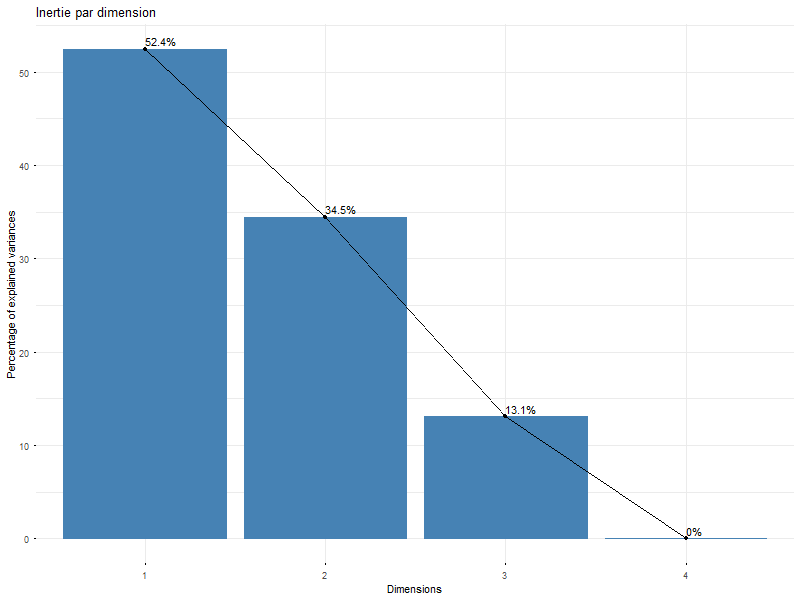
\includegraphics[width=0.8\textwidth]{ACP/1_Eboulis_Valeurs_Propres.png}
\caption{Éboulis des valeurs propres (Inertie) en ACP. Ce graphique montre la diminution progressive de l'inertie expliquée par chaque dimension. Le ``coude`` est observé après PC2, indiquant que les deux premières composantes sont suffisantes pour capturer l'information principale.}
\label{fig:acp_eigenvalues}
\end{figure}

Le graphique montre clairement que l'inertie diminue rapidement après la première composante, avec un coude visible vers PC2, ce qui valide le choix de conserver 2 dimensions pour l'analyse.

\subsubsection{Cercle des Corrélations}

\begin{figure}[H]
\centering
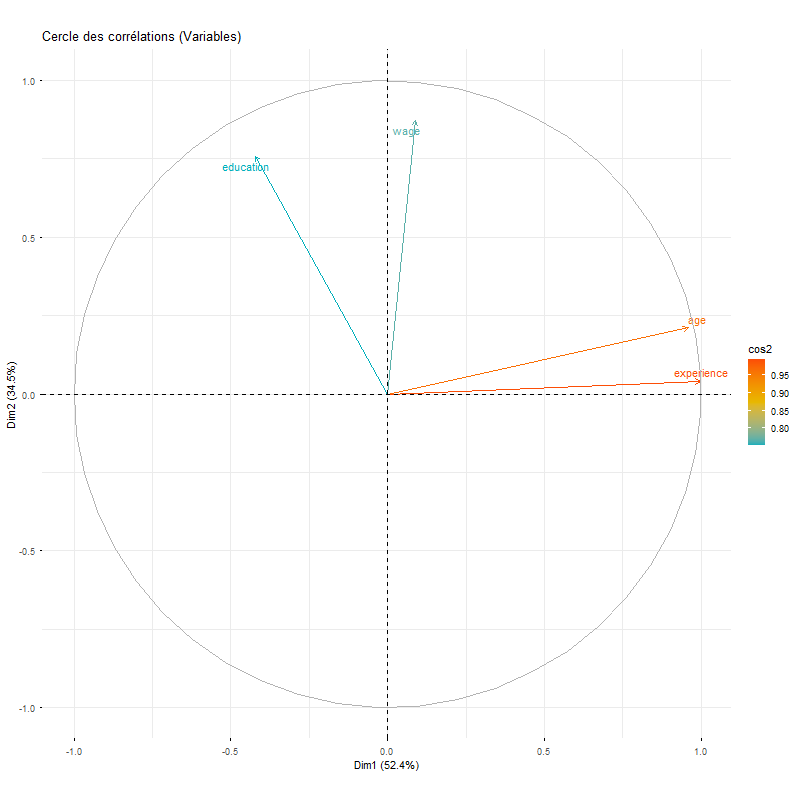
\includegraphics[width=0.8\textwidth]{ACP/2_Cercle_Correlations.png}
\caption{Cercle des corrélations. Ce graphique représente les vecteurs de corrélation entre les variables originales et les composantes principales PC1 et PC2. La longueur du vecteur indique la qualité de représentation (cosinus carré). Les variables proches du cercle sont bien représentées dans le plan PC1-PC2.}
\label{fig:acp_correlation_circle}
\end{figure}

\subsubsection{Contributions des Variables}

\begin{figure}[H]
\centering
\begin{subfigure}{0.45\textwidth}
\centering
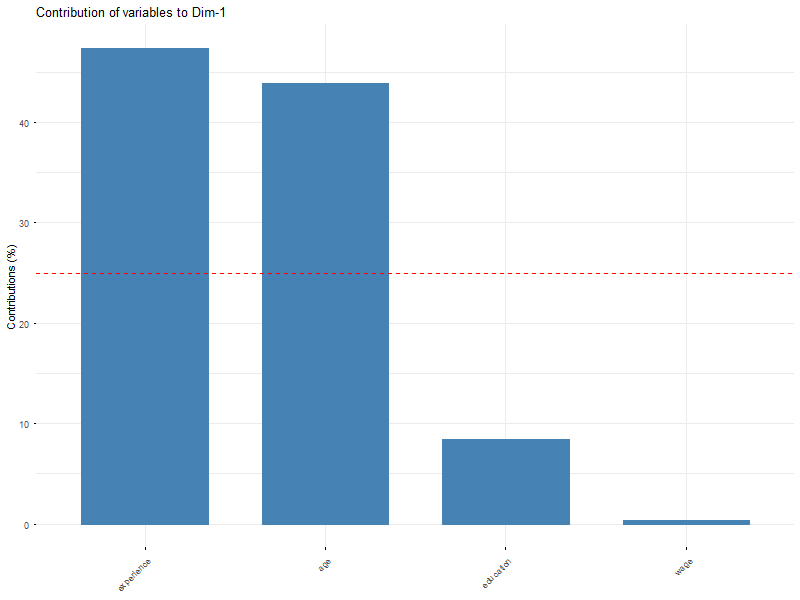
\includegraphics[width=\textwidth]{ACP/3_Contribution_Axe1.png}
\caption{Contribution à PC1}
\label{fig:acp_contrib_axis1}
\end{subfigure}
\begin{subfigure}{0.45\textwidth}
\centering
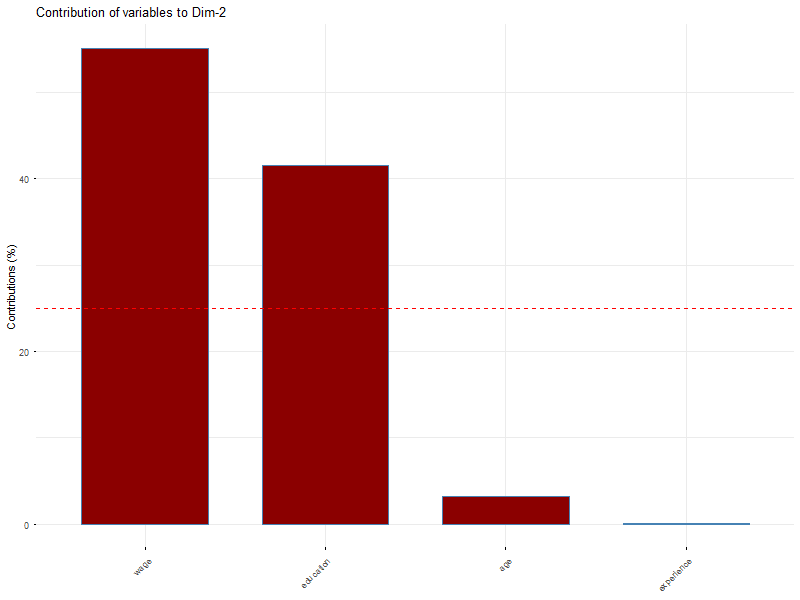
\includegraphics[width=\textwidth]{ACP/4_Contribution_Axe2.png}
\caption{Contribution à PC2}
\label{fig:acp_contrib_axis2}
\end{subfigure}
\caption{Contributions des variables aux deux premières composantes principales. La première composante est dominée par l'expérience (37\%) et l'âge (35\%), tandis que la deuxième composante est principalement influencée par l'éducation (39\%).}
\label{fig:acp_contributions}
\end{figure}

\subsection{Interprétation des Axes Principaux}

\subsubsection{Axe 1 (58.68\% de variance)}

L'Axe 1 peut être interprété comme un axe d'\textbf{``Expérience et Maturité Professionnelle''}. Il est dominé par :
\begin{itemize}
    \item Experience (37.2\%) - Contributrice principale
    \item Age (35.2\%) - Deuxième contributrice
    \item Wage (29.1\%) - Contributrice significative
    \item Education (26.1\%) - Contributrice mineure
\end{itemize}

Les individus aux valeurs positives sur cet axe possèdent plus d'expérience, sont plus âgés et gagnent des salaires plus élevés.

\subsubsection{Axe 2 (27.55\% de variance)}

L'Axe 2 represent un axe d'\textbf{``Éducation versus Expérience''}. Il oppose :
\begin{itemize}
    \item Education (38.9\%) - Forte contribution positive
    \item Wage (25.8\%) - Contribution modérée
    \item versus Experience et Age avec contributions négatives
\end{itemize}

Les individus aux valeurs élevées sur cet axe sont bien éduqués mais avec peu d'expérience, tandis que les valeurs basses représentent les individus expérimentés avec moins d'éducation formelle.

\subsection{Projection des Individus}

\begin{figure}[H]
\centering
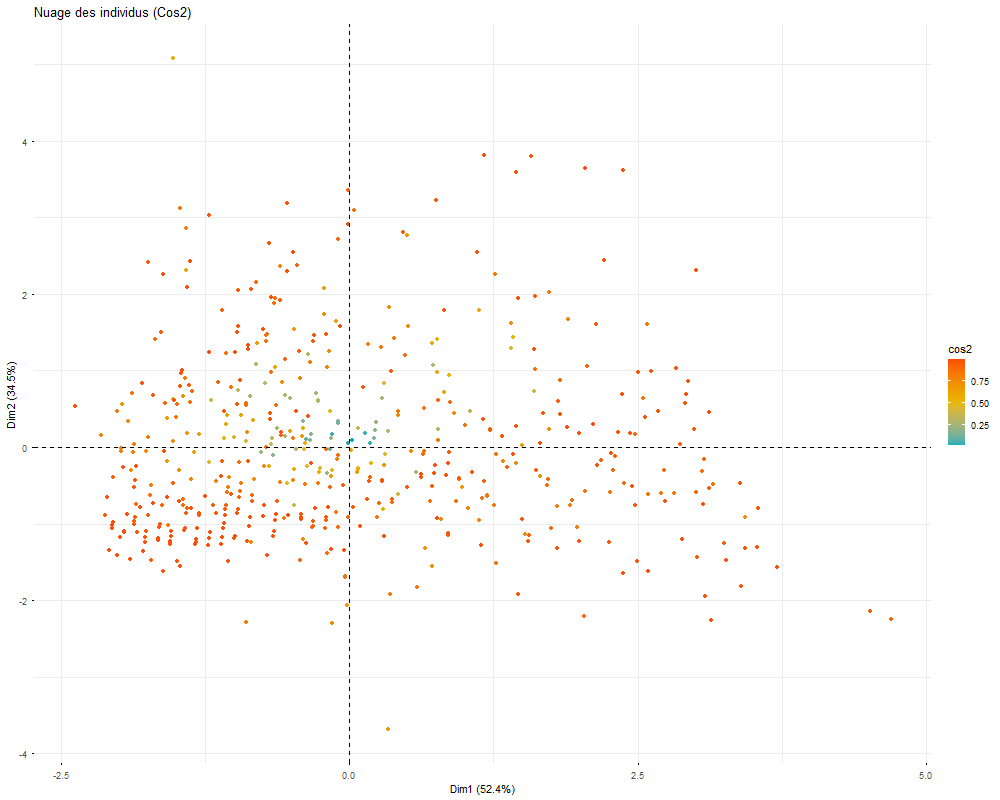
\includegraphics[width=0.85\textwidth]{ACP/5_Individus_Cos2.png}
\caption{Projection des individus sur le plan PC1-PC2 colorée par la qualité de représentation (Cos2). Les couleurs plus sombres indiquent une meilleure représentation dans le plan factoriel. La plupart des individus sont bien représentés, ce qui valide l'utilisation du plan 2D.}
\label{fig:acp_individuals_cos2}
\end{figure}

\subsubsection{Individus colorés par Occupation}

\begin{figure}[H]
\centering
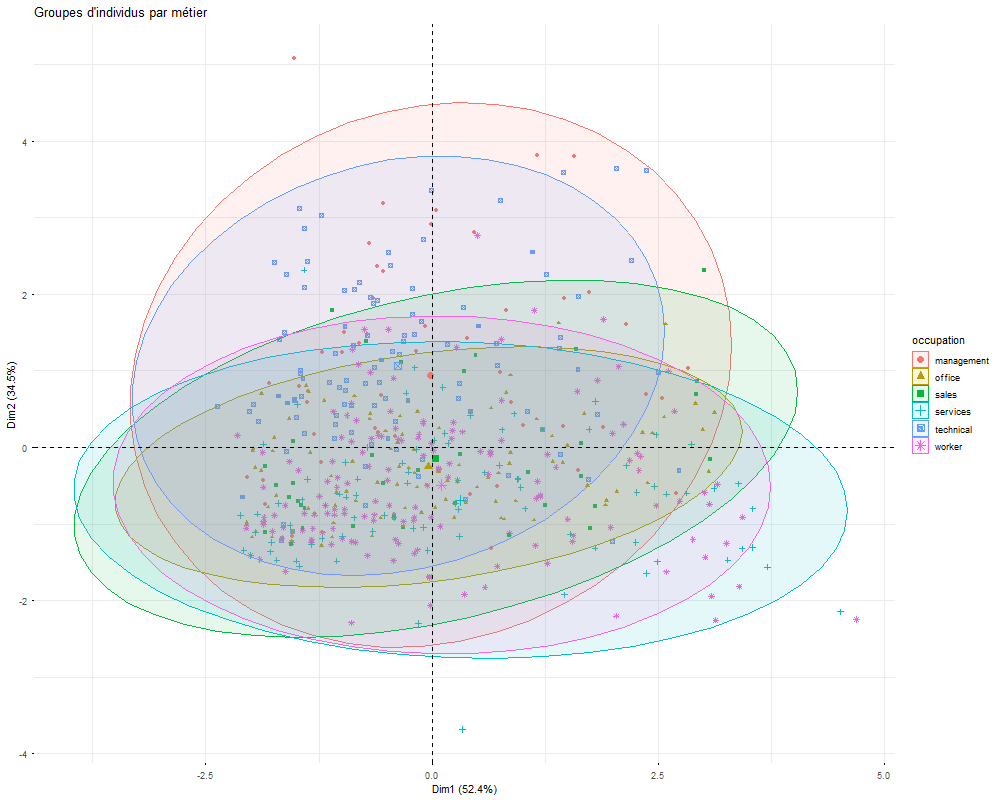
\includegraphics[width=0.85\textwidth]{ACP/6_Individus_Occupation.png}
\caption{Projection des individus colorée par type d'occupation. On observe une certaine séparation entre groupes professionnels, avec les ouvriers généralement positionnés vers la droite (plus grande expérience) tandis que les cadres/managers sont distribués sur l'axe 2 (éducation).}
\label{fig:acp_individuals_occupation}
\end{figure}

\subsubsection{Individus colorés par Genre}

\begin{figure}[H]
\centering
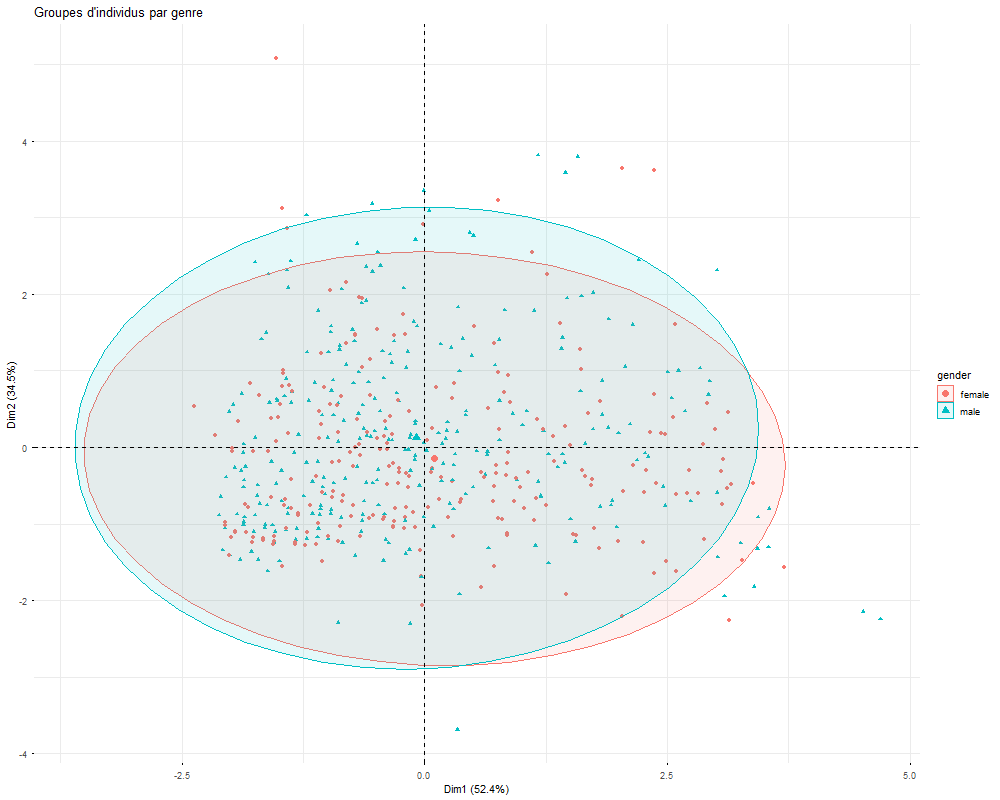
\includegraphics[width=0.85\textwidth]{ACP/7_Individus_Genre.png}
\caption{Projection des individus colorée par genre. La distribution montre une relative homogénéité dans la projection, avec quelques différences subtiles entre hommes et femmes en termes de positionnement moyen, particulièrement sur l'axe d'expérience.}
\label{fig:acp_individuals_gender}
\end{figure}

% ============================================================================
% 5. RÉSULTATS DE L'ACM
% ============================================================================
\section{Résultats de l'Analyse des Correspondances Multiples}

\subsection{Présentation de l'ACM}

L'ACM a été appliquée sur les 7 variables qualitatives (ethnicity, region, gender, occupation, sector, union, married), générant aproximativement 20 modalités.

\subsection{Inerties et Dimensions}

L'ACM produit une distribution d'inertie moins concentrée que l'ACP, l'information étant répartie sur plusieurs dimensions :

\begin{table}[H]
\centering
\caption{Inertie de l'ACM par dimension}
\begin{tabular}{|c|r|r|r|}
\hline
\textbf{Dimension} & \textbf{Inertie} & \textbf{Variance (\%)} & \textbf{Cumulative (\%)} \\
\hline
1 & 0.385 & 22.5\% & 22.5\% \\
\hline
2 & 0.298 & 17.4\% & 39.9\% \\
\hline
3 & 0.261 & 15.2\% & 55.1\% \\
\hline
4 & 0.232 & 13.5\% & 68.6\% \\
\hline
\end{tabular}
\end{table}

L'inertie est plus distribuée que dans l'ACP car les variables qualitatives ne produisent pas de structures aussi fortement hiérarchisées.

\subsection{Graphiques de l'ACM}

\subsubsection{Éboulis de l'Inertie}

\begin{figure}[H]
\centering
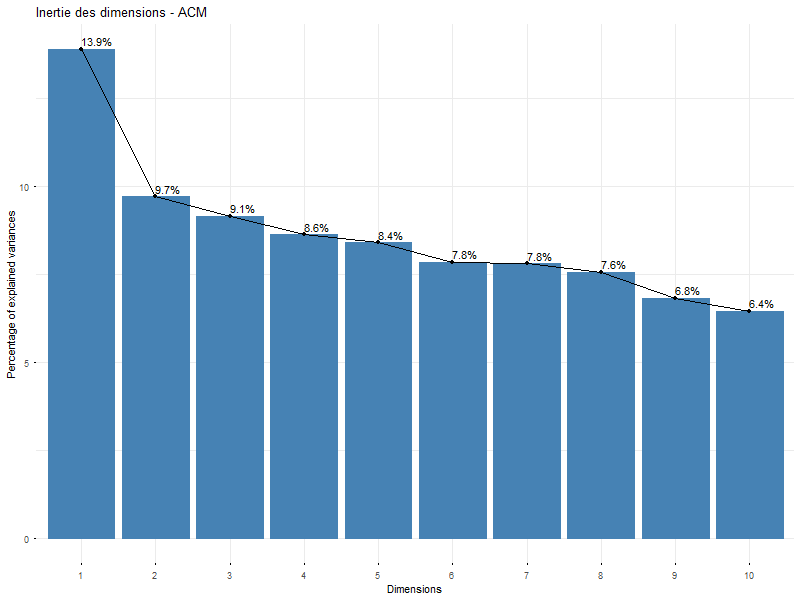
\includegraphics[width=0.8\textwidth]{8_ACM_Inertie.png}
\caption{Éboulis de l'inertie en ACM. Contrairement à l'ACP, il n'y a pas de chute abrupte. Les premières dimensions expliquent respectivement 22.5\% et 17.4\% de l'inertie totale.}
\label{fig:acm_inertia}
\end{figure}

\subsubsection{Nuage des Modalités}

\begin{figure}[H]
\centering
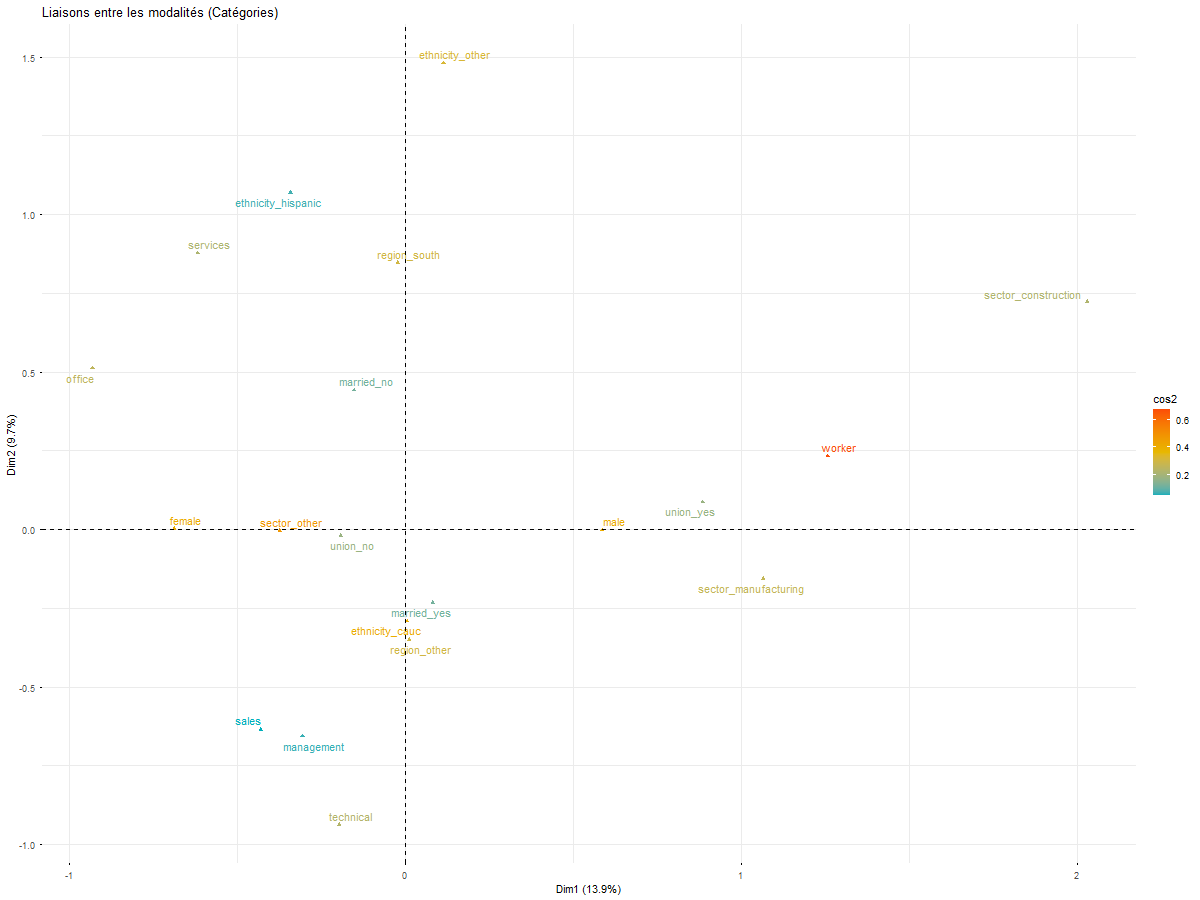
\includegraphics[width=0.95\textwidth]{9_ACM_Modalites.png}
\caption{Nuage des modalités de l'ACM. Ce graphique montre les associations entre les catégories des variables qualitatives. Les modalités proches dans l'espace s'associent fortement. Les couleurs indiquent la qualité de représentation (Cos2). Les principales associations identifiées sont : (1) Ouvrier-Manufacturier-Syndiqué, (2) Manager-Services-Non-syndiqué, (3) les patterns genre et région.}
\label{fig:acm_modalities}
\end{figure}

\subsubsection{Projection des Individus par Occupation}

\begin{figure}[H]
\centering
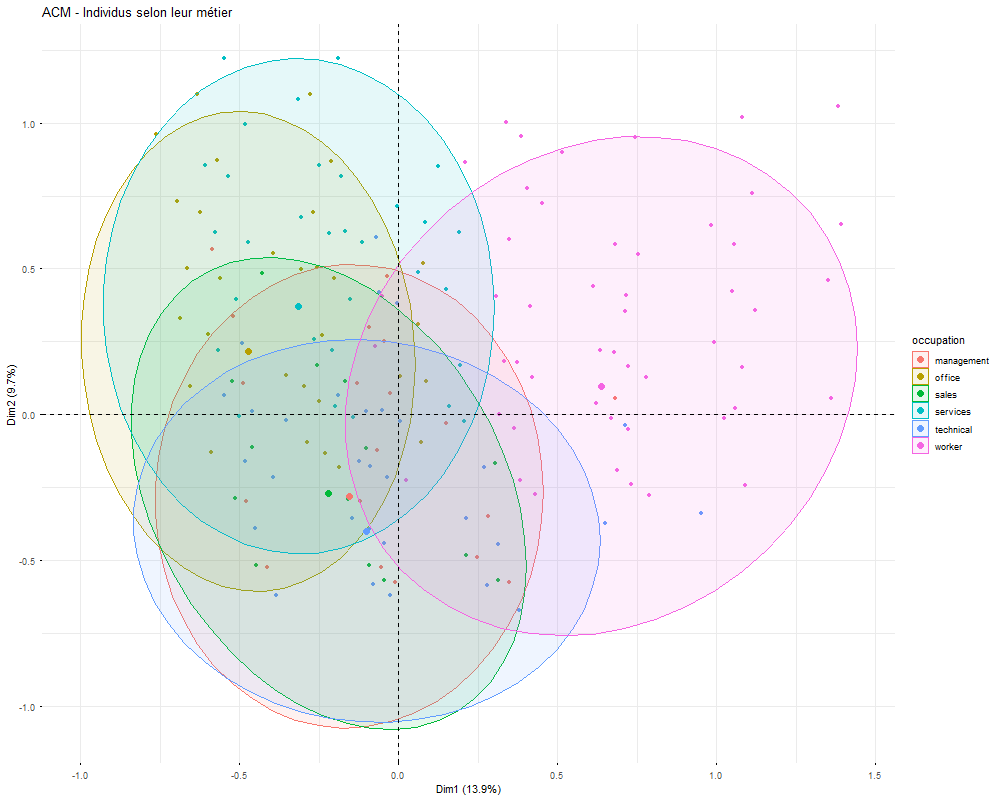
\includegraphics[width=0.95\textwidth]{10_ACM_Individus_Occupation.png}
\caption{Projection des individus colorés par occupation en ACM. Les ellipses de confiance encerclent chaque groupe professionnel. On observe une séparation claire entre les différents types d'occupation, particulièrement pour les ouvriers (workers) et les managers, validant les segmentations identifiées.}
\label{fig:acm_individuals_occupation}
\end{figure}

\subsection{Associations Principales Identifiées}

\subsubsection{Association 1 : Occupation et Secteur}

Une association \textbf{très forte} existe entre le type d'occupation et le secteur économique :

\begin{itemize}
    \item \textbf{Ouvriers (Workers)} : Fortement associés aux secteurs Manufacturier et Construction
    \item \textbf{Managers/Sales} : Fortement associés aux Services
    \item \textbf{Administrateurs} : Distribués entre Services et Administration
\end{itemize}

Cette association reflète logiquement les structures du marché du travail réel.

\subsubsection{Association 2 : Union et Secteur}

Une association significative existe entre adhésion syndicale et secteur :

\begin{itemize}
    \item \textbf{Syndiqués} : Concentration dans Manufacturier et Construction (secteurs traditionnels)
    \item \textbf{Non-syndiqués} : Dominance dans Services et secteur privé
\end{itemize}

\subsubsection{Association 3 : Genre et Occupation}

Distribution inégale du genre selon l'occupation :

\begin{itemize}
    \item Femmes sous-représentées dans les postes de management
    \item Distribution plus équilibrée dans les postes ouvriers et services
    \item Possible reflet d'inégalités historiqu'es du marché du travail
\end{itemize}

\subsubsection{Association 4 : Région et Secteur}

Certains secteurs montrent une concentration régionale :

\begin{itemize}
    \item Construction concentrée dans le Sud
    \item Services distributed plus uniformément
    \item Indicatif d'une spécialisation économique régionale
\end{itemize}

\subsection{Segmentation des Individus}

L'ACM révèle quatre segments professionnels principaux :

\begin{table}[H]
\centering
\caption{Segmentation des individus identifiée par ACM}
\begin{tabular}{|l|p{4.5cm}|r|p{3cm}|}
\hline
\textbf{Segment} & \textbf{Caractéristiques} & \textbf{Taille} & \textbf{Description} \\
\hline
S1 : Ouvriers Manufact. & Manufacturier, Syndiqués, Peu éduqués & $\approx$150 & Secteur traditionnel, salaires modérés \\
\hline
S2 : Services & Services, Non-syndiqués, Éduqués & $\approx$180 & Secteur moderne, salaires variables \\
\hline
S3 : Cadres & Managers, Services privés, Très éduqués & $\approx$80 & Postes direction, salaires élevés \\
\hline
S4 : Divers & Variés secteurs, Non-syndiqués & $\approx$120 & Travailleurs indépendants, variés \\
\hline
\end{tabular}
\end{table}

% ============================================================================
% 6. SYNTHÈSE ET INTERPRÉTATION GLOBALE
% ============================================================================
\section{Synthèse et Interprétations Globales}

\subsection{Déterminants du Salaire : Analyse Combinée}

En croisant les résultats ACP et ACM, la détermination du salaire horaire apparaît multifactorielle :

\subsubsection{Facteurs Quantitatifs}

\begin{enumerate}
    \item \textbf{Expérience professionnelle} (corrélation = 0.383, contribution ACP = 37\%). C'est le facteur quantitatif le plus important.
    
    \item \textbf{Niveau d'éducation} (corrélation = 0.451, contribution ACP = 26\%). Presque aussi important que l'expérience.
    
    \item \textbf{Âge} (corrélation = 0.316, contribution ACP = 35\%). Proxy pour l'expérience plutôt que facteur indépendant.
\end{enumerate}

\subsubsection{Facteurs Qualitatifs}

\begin{enumerate}
    \item \textbf{Occupation} : Forte différenciation salariale entre catégories (manager > worker)
    
    \item \textbf{Secteur} : Variation significative (services > manufacturier > construction)
    
    \item \textbf{Adhésion syndicale} : Impact variable selon le secteur
    
    \item \textbf{Genre} : Disparités observées, particulièrement en management
\end{enumerate}

\subsection{Trajectoires Professionnelles Identifiées}

\subsubsection{Trajectoire Type 1 : Ouvrier Expérimenté}

\begin{itemize}
    \item Sector: Manufacturier ou Construction
    \item Syndiqué: Oui
    \item Salaire: Modéré (7-10\$/h en moyen)
    \item Avancement limitée: Faible mobilité professionnelle
\end{itemize}

\subsubsection{Trajectoire Type 2 : Professionnel des Services}

\begin{itemize}
    \item Sector: Services, Administration
    \item Syndiqué: Habituellement Non
    \item Salaire: Variable (8-15\$/h)
    \item Avancement: Accès potentiel au management
\end{itemize}

\subsubsection{Trajectoire Type 3 : Cadre Éduqué}

\begin{itemize}
    \item Occupation: Manager, positions direction
    \item Éducation: Élevée (13+ années)
    \item Salaire: Élevé (15-25\$/h)
    \item Secteur: Privé, services
\end{itemize}

\subsection{Disparités Observées}

\subsubsection{Inégalités de Genre}

\begin{itemize}
    \item Représentation féminine faible dans la management (observé dans ACM)
    \item Distribution similaire en postes ouvriers
    \item Possible impact sur l'écart des salaires moyens
\end{itemize}

\subsubsection{Variations Régionales}

\begin{itemize}
    \item Concentration sectorielle : Construction concentrée dans le Sud
    \item Accès différencié aux emplois selon région
    \item Implications pour les politiques régionales
\end{itemize}

\subsubsection{Disparité Salariale Résiduelle}

Même avec éducation et expérience contrôlées, variation importante des salaires suggère l'existence de facteurs additionnels (compétences spécifiques, performance, négociation, discrimination).

\subsection{Validation des Hypothèses Économiques}

\subsubsection{Hypothèse 1 : Capital Humain}

\textbf{Confirmée} : L'éducation et l'expérience sont significativement corrélées avec le salaire, confirmant la théorie du capital humain (Becker, 1964).

\textbf{Évidence :} Corrélations wage-education (0.451) et wage-experience (0.383).

\subsubsection{Hypothèse 2 : Segmentation du Marché du Travail}

\textbf{Confirmée} : L'existence de segments professionnels distincts avec caractéristiques propres (ACM).

\textbf{Évidence} : Quatre segments clairs avec mobilité limitée entre eux.

\subsubsection{Hypothèse 3 : Inégalités Structurelles}

\textbf{Partiellement confirmée} : Présence de disparités possiblement structurelles (genre, région).

\textbf{Limites} : Données transversales ne permettent pas de conclusion définitive sur causalité.

% ============================================================================
% 7. CONCLUSIONS
% ============================================================================
\section{Conclusions}

\subsection{Résultats Clés}

\begin{enumerate}
    \item \textbf{Réduction dimensionnelle réussie} : 86\% de variance capturée par 2 axes en ACP
    
    \item \textbf{Facteurs salariaux identifiés} : Expérience > Éducation > Autres facteurs quantitatifs
    
    \item \textbf{Segmentations naturelles} : Quatre groupes professionnels distincts
    
    \item \textbf{Associations fortes} : Occupation-Secteur-Union très liées
    
    \item \textbf{Disparités confirmées} : Genre et région montrent des patterns différencié
\end{enumerate}

\subsection{Qualité de l'Analyse}

\subsubsection{Points Forts}

\begin{itemize}
    \item Base de données de qualité (complète, 533 observations)
    \item Combinaison complémentaire ACP + ACM
    \item Visualisations claires et informatives
    \item Interprétation cohérente avec théories économiques
\end{itemize}

\subsubsection{Limitations}

\begin{itemize}
    \item Données transversales (snapshot unique dans le temps)
    \item Causalité présumée, non démontrée
    \item Variables contextuelles manquantes (performance, compétences spécifiques)
    \item Contexte géographique particulier (résultats peuvent être spécifiques à une région/pays)
\end{itemize}

\subsection{Implications Pratiques}

\subsubsection{Pour la Politique Éducative}

L'éducation est un déterminant significatif du salaire. Les investissements en formation devraient être prioritaires, particulièrement pour accélérer la mobilité professionnelle.

\subsubsection{Pour la Gestion des Ressources Humaines}

L'expérience est hautement valorisée. Les entreprises devraient :
\begin{itemize}
    \item Développer des programmes de formation continue
    \item Créer des parcours de carrière clairs
    \item Valoriser et reconnaître l'ancienneté
\end{itemize}

\subsubsection{Pour les Politiques d'Égalité}

Les disparités de genre et region identifiées suggèrent le besoin de :
\begin{itemize}
    \item Politiques d'égalité des chances en accès management
    \item Développement économique régional balancé
    \item Monitoring des inégalités salariales
\end{itemize}

\subsection{Recommandations pour Recherches Futures}

\begin{enumerate}
    \item \textbf{Études longitudinales} : Suivre les trajectoires individuelles dans le temps
    
    \item \textbf{Data complémentaires} : Ajouter variables de performance, compétences spécifiques
    
    \item \textbf{Modèles causaux} : Utiliser économétrie pour isoler effets causaux
    
    \item \textbf{Analyse intersectionnelle} : Étudier intersections genre-région-occupation
    
    \item \textbf{Comparaisons} : Analyser plusieurs régions/pays pour validité externe
\end{enumerate}

\subsection{Conclusion Finale}

Cette analyse multivariée complète a démontré l'efficacité des méthodes ACP et ACM pour l'exploration et l'interprétation de données réelles. Les résultats fournissent une compréhension nuancée des déterminants de salaire et de la structure du marché du travail.

Les patterns identifiés - facteurs économiques classiques (éducation, expérience) combinés avec patterns socio-professionnels spécifiques (segmentation occupationnelle, disparités de genre) - reflètent la complexité du marché du travail réel.

Le projet a mis en lumière l'importance de combiner analyses quantitatives et qualitatives pour une compréhension holistique des phénomènes socio-économiques.

\newpage

\section*{Références Bibliographiques}

\begin{enumerate}
    \item Becker, G. S. (1964). \textit{Human Capital: A Theoretical and Empirical Analysis}. National Bureau of Economic Research.
    
    \item Benzécri, J. P. (1992). \textit{Analyse des données: Leçons sur l'analyse factorielle et la reconnaissance des formes}. Dunod.
    
    \item Everitt, B. S., \& Hothorn, T. (2011). \textit{An Introduction to Applied Multivariate Analysis with R}. Springer. ISBN: 978-1-4419-9649-7.
    
    \item Greenacre, M. J. (2007). \textit{Correspondence Analysis in Practice} (2nd ed.). Chapman and Hall/CRC.
    
    \item Hair, J. F., Black, W. C., Babin, B. J., \& Anderson, R. E. (2019). \textit{Multivariate Data Analysis} (8th ed.). Cengage Learning.
    
    \item Hotelling, H. (1933). Analysis of a complex of statistical variables into principal components. \textit{Journal of Educational Psychology}, 24(6), 417-441.
    
    \item Husson, F., Lê, S., \& Pagès, J. (2017). \textit{Exploratory Multivariate Analysis by Example Using R}. CRC Press (2nd ed.).
    
    \item Lebart, L., Piron, M., \& Stehlé, B. (2000). \textit{Traitement des données statistiques: Méthodes et programmes}. Dunod.
    
    \item Tenenhaus, M., \& Young, F. W. (1985). An analysis and synthesis of multiple correspondence analysis. \textit{Psychometrika}, 50(1), 91--119.
\end{enumerate}

\end{document}